% \textit{\textbf{The following section formatting is \textbf{optional}, you can also define sections as you deem fit.
% \\
% Focus on what future researchers or practitioners would find useful for reproducing or building upon the paper you choose.\\
% For more information of our previous challenges, refer to the editorials \cite{Sinha:2022,Sinha:2021,Sinha:2020,Pineau:2019}.
% }}
\newcommand{\norm}[1]{\left\Vert #1 \right\Vert}
\newcommand{\Z}{\mathbb{Z}}
\newcommand{\Q}{\mathbb{Q}}
\newcommand{\N}{\mathbb{N}}
% \newcommand{\C}{\mathbb{C}}
\newcommand{\R}{\mathbb{R}}


\renewcommand{\P}{\mathbb{P}}
\newcommand{\Id}{\operatorname{Id}}

\newcommand{\calS}{\mathcal{S}}
\newcommand{\calP}{\mathcal{P}}
\newcommand{\calF}{\mathcal{F}}
\newcommand{\calL}{\mathcal{L}}
\newcommand{\calV}{\mathcal{V}}


\newcommand{\abs}[1]{\left\vert #1 \right\vert}
% \newcommand{\norm}[1]{\left\Vert #1 \right\Vert}
\newcommand{\set}[1]{\left\lbrace #1\right\rbrace}
\newcommand{\sse}{\subseteq}
\newcommand{\sprod}[1]{\left\langle #1 \right\rangle}
\section{Introduction}
Image classification models have grown exponentially in size and prevalence over the last few years. This, along with their "black box" nature, highlights the challenge of explaining the results and decisions made by these image classification models in a more interpretable manner for their human operators. There has been considerable research in this domain (\cite{macdonald2019rate, selvaraju2017grad, sundararajan2017axiomatic, smilkov2017smoothgrad, springenberg2014striving, LRP, ribeiro2016should}) to generate importance mask on the pixel space. However, they frequently result in sparse and shaky explanations.

This paper presents a novel explanation method that operates in the wavelet domain of images instead of the conventional pixel space and aims to extract relevant piece-wise smooth parts of an image. This is achieved by demanding sparsity in the wavelet domain, which can further result in piece-wise smooth explanations.


\section{Scope of Reproducibility}
\label{sec:claims}
The paper that we reproduce addresses the difficulties associated with pixel-based explanation methods stemming from the fact that they produce pixel-sparse explanations that incur higher levels of distortion than the suggested CartoonX method. 
In our reproducibility study, we reproduce the results of the original work, assess the claims made, and present several additional experiments to extend the previous work. In short, we present the following:
\begin{itemize}
    \item Through the reproduction of qualitative and quantitative results, we verify their claim that  CartoonX gives better explanations when compared to other pixel-based explanation methods. 
    \item We extend the previous paper through experimentation with the obfuscation method to improve the distortion values achieved.
    \item We extend the applications of CartoonX to the domains of semantic segmentation and object detection.
    \item We further conduct an ablation study on the use of CartoonX over several different deep neural network architectures. 
\end{itemize}
In order to examine and explain the points touched upon, the report first discusses the CartoonX methodology in more detail in \autoref{sec:cartoonx}, followed by \autoref{sec:methodology}, where the reproduction and extensions made are described. After this, we discuss the results of the reproducibility study and extensions in \autoref{sec:results}, followed by the discussion in \autoref{sec:discussion}. 


\section{CartoonX}\label{sec:cartoonx}
CartoonX is a model-agnostic explanation method that can extract explanations from image classifiers via the RDE(rate-distortion explanation)framework. We briefly summarize the main ideas of this methodology in this section.\\
\\
Let $\Phi:\R^n\to\R^m$ be a deep neural network and $x\in \R^n $ a data point with a data representation $x =f(h_1,...,h_k)$ where $f$ is the inverse discrete wavelet transform operator. Here, coefficients $[h_i]_{i=1}^n$ can be obtained by applying discrete wavelet transform on $x$. Let the mask be $s\in[0,1]^k$,  $\calV$ be a probability distribution over $\prod_{i=1}^k\R^{c}$. Then the \emph{obfuscation} of $x$ concerning $s$ and $\mathcal{V}$ is defined as
$y \coloneqq f(s\odot h + (1-s)\odot v)$. Thus the expected distortion is given by
$$
D(x,s,\mathcal{V}, \Phi)\coloneqq \mathop{\mathbb{E}}_{v\sim \mathcal{V}} \Big[ d\Big(\Phi(x), \Phi(y)\Big)\Big],
$$
where $d$ is a measure of distortion and $\Phi$ represent the model decision .The aim is to find a sparse mask $s$ and minimize $D(x,s,\mathcal{V}, \Phi)$. This results in the following constrained optimization problem.
\begin{align}\label{eq:relax_problem_ell1}
    \min_{s\in [0,1]^k} \quad D(x,s,\mathcal{V}, \Phi) + \lambda \|s\|_1,
\end{align}

This objective can be optimized via stochastic gradient descent (SGD). Also note that they approximate $D(x,s,\mathcal{V}, \Phi)$ with i.i.d. samples from $v\sim \calV$ . Finally they visualize the mask $s$ as a piece-wise smooth image in pixel
space by multiplying the mask with the DWT coefficients of the greyscale image, followed by applying inverse DWT.


\section{Methodology}\label{sec:methodology}
In order to replicate the results generated by the original authors, we used the script provided by the authors. Their step-by-step documentation detailing how to install specific dependencies, such as the {\it PyTorch Wavelets} module, made it relatively easy to reproduce some of their qualitative results for the CartoonX and Pixel RDE implementations. However, the other explainability methods shown in the qualitative comparisons required additional implementation. Additional scripts were also required for the sensitivity analysis. \\
Apart from this, we also attempt to extend the applications of CartoonX to Semantic Segmentation and Object Detection tasks. Semantic segmentation deals with assigning a class
to each pixel of an image. Since this classification problem is applied to each pixel,
it is fairly straightforward to plug CartoonX to visualize the explanations. Object detection, however, is more difficult with assigning bounding boxes around
objects in an image and their identification. Specifically, in our experiment, we
work with the YOLO algorithm. Applying CartoonX directly on YOLO wouldn’t work because with every update of the wavelet mask, the network outputs change, and so the Non‐
max suppression module of the YOLO ends up with a different set of objects every update. This makes computing the loss difficult. To circumvent this, we calculated the loss among the predictions of the perturbed and the non‐
perturbed input just before the Non‐max suppression stems. This trick works well in practice, as we will see from the results.\\

\subsection{Model descriptions}
The paper predominantly used the Pixel RDE and CartoonX methodologies, where PixelRDE was used as a baseline methodology. Two pre-trained models were also used to assess the explanation capabilities of the two methodologies. These were the VGG-16 \cite{simonyan2014very} and MobileNetv3-small \cite{howard2019searching} models pre-trained on ImageNet, obtained via PyTorch. \\ 
The CartoonX method implemented within the original paper stems from the contributions made by \cite{macdonald2019rate} and \cite{heiss2020distribution} via rate distortion explanations (RDE). This RDE methodology was then applied not in the pixel domain but in the Wavelet basis of the images to use the more relevant, smooth portions of the signal. 

\subsection{Datasets}
The original paper considers random ImageNet \cite{deng2009imagenet} samples as its data for producing the results. Specifically, they computed explanations for 100 random ImageNet samples for comparison between different methods. To make the comparison fair, they resize the images to $256 \times 256$ before passing them to models.  

\subsection{Hyperparameters}
The original paper and we use the same hyperparameter setting. We use Adam optimizer, a learning rate of $\epsilon=0.001$, $L=64$ adaptive Gaussian noise samples, and $N=2000$ steps. We specify the sparsity level in terms of the number of mask entries $k$, i.e., by choosing the product $\lambda k$. For CartoonX, we consider $\lambda k \in [20, 80]$, whereas we consider $\lambda k \in [3, 20]$ for Pixel RDE, as it typically requires a smaller sparsity level than CartoonX. When using the CartoonX methodology, the Daubechies 3 (db3) method was the baseline wavelet system, with a discrete wavelet transform scale of 5.

\subsection{Computational requirements}

The experiments were conducted using several types of CUDA-based GPUs, namely the RTX 3060 and the GTX 2060Ti. The qualitative results ran on the RTX 3060 consisted of the results in \autoref{fig:results-qual-1}, \autoref{fig:mis-classification}, \autoref{fig:vgg-16}, \autoref{fig:sensitivity-analysis}, \autoref{fig:quantitative-results-7c}, and all of \autoref{app:qualitative-results}. The quantitative results executed on the RTX 3060 shown in \autoref{fig:quantitative-results-7c} required the most computation time to be allotted, totaling 36.25 hours. 
\subsection{Reproduction Setup}
Our experimental setup is closely based on the original paper. For verifying the quantitive analysis in the paper, we show three plots (i) between distortion and non-randomized relevant components and (ii) between distortion and randomized relevant components. (iii) between distortion and non-sparsity. We also plot an accuracy vs. non-randomized relevant component to understand the first plot better. 
\subsection{Extension Setup}
\subsubsection{Obfuscation Deviation Scaling}
As an extension to the original paper, a simple improvement to the obfuscation method was devised. This improvement took the original standard deviations of the individual wavelets derived from an image. It scaled them according to their resolution, where the scaling was done linearly, with the lowest wavelet being weighted the highest and the highest being weighted the lowest. This scaling depended on the number of wavelet components used within the Daubechies (db3) method. The equation $\sigma_{i_{new}} =\frac{i}{J}\sigma_{i_{old}}$ is used as the scaling for each i wavelet deviation out of the total of J wavelets. The inverse of this was used as well $\sigma_{i_{new}} =\frac{J-i}{J}\sigma_{i_{old}}$. This scaling was also applied inversely and exponentially to determine a method with the lowest amount of distortion while still producing qualitatively good results. The equation $\sigma_{i_{new}} = 2^{\frac{-i}{J}}\sigma_{i_{old}}$ was used for the inverse exponential, where J denoted the number of wavelets, and i is the index of a particular wavelet, starting with 1. 
\subsubsection{Application on Semantic Segmentation and Object Detection}
We use a pretrained DeepLabV3 model with a ResNet-50 backbone to experiment with Semantic Segmentation and a pretrained YOLO-V5 network for Object detection.
\section{Results}
\label{sec:results}
The qualitative results aligned with the initial paper's qualitative results. However, the same cannot be said for the quantitative results generated using the same hyperparameters specified within the paper.

\subsection{Reproducibility Study}
After completing the reproduction process of this paper, the qualitative results were similar to those achieved by the original paper. This applies to both the CartoonX and PixelRDE implementations, which are displayed in \autoref{fig:results-qual-1} where the original hyperparameters MobileNetv3-small model. Additional results can be found in \autoref{app:qualitative-results}.

\begin{figure}[H]
    \centering
    \includegraphics[width=0.6\textwidth]{images/qualitative_ims/correct_qualitative_ims/tench.png}
    \caption{Qualitative Results with original hyperparameters}
    \label{fig:results-qual-1}
\end{figure}
When compared to the qualitative results generated via the original method described within the paper, several similarities are apparent for both the PixelRDE and CartoonX methodologies. For the PixelRDE method, correctly classified image explanations are mostly black, save for some outlines and highlighted key features. In contrast, the outline remains clear for the CartoonX explanation method, as do key defining features. \\
Qualitative results for misclassified images were also generated, shown in \autoref{fig:mis-classification}.
\begin{figure}[ht]
    \centering
    \includegraphics[width=0.6\textwidth]{images/qualitative_ims/incorrect_qualitative/vase.png}
    \caption{Image of an Indian Cobra misclassified as a vase.}
    \label{fig:mis-classification}
\end{figure}
This methodology's qualitative results were also explored using the VGG16 model, resulting in \autoref{fig:vgg-16}.
\begin{figure}[ht]
    \centering
    \includegraphics[width=0.6\textwidth]{images/qualitative_ims/vgg_qualitative/vgg_jay_new.png}
    \caption{Images resulting from the use of the VGG16 model.}
    \label{fig:vgg-16}
\end{figure}

The results from the qualitative sensitivity analysis are displayed in \autoref{fig:sensitivity-analysis}. The sensitivity analysis used the hyperparameters specified in both the figures and the text provided. No additional tweaking was required to complete these experiments, except for a minor addition to what is provided in the script, as the weighted-L2 distortion measure required. 

\begin{figure}[ht]

\centering
\subfloat[]{\includegraphics[width=0.45\textwidth]{images/qualitative_ims/8a.png}}\hfil
\subfloat[]{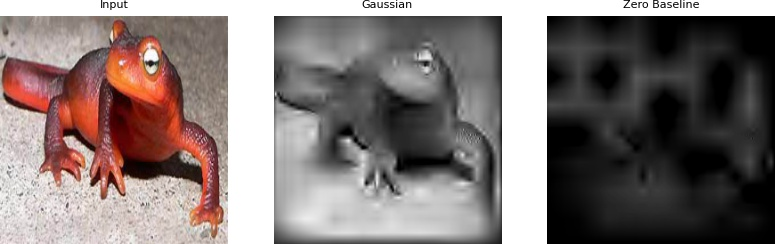
\includegraphics[width=0.45\textwidth]{images/qualitative_ims/8b.JPEG}}


\subfloat[]{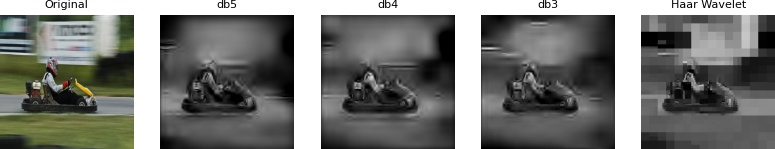
\includegraphics[width=0.45\textwidth]{images/qualitative_ims/8c.JPEG}}\hfil   
\subfloat[]{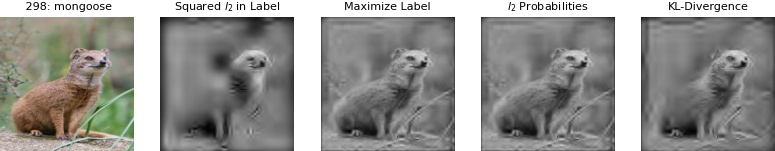
\includegraphics[width=0.45\textwidth]{images/qualitative_ims/8d.JPEG}}

\caption{Qualitative Sensitivity Analysis}\label{fig:sensitivity-analysis}
\end{figure}


When reproducing the quantitative analysis, it was uncovered that several quantitative plots used hyperparameters that were not properly included. The initial assumption was to use 2000 steps, as this was the specified number of steps for both the PixelRDE and CartoonX methodologies. However, this was deemed an unfair assessment, as some methods used 100 steps. One hundred steps were used to compare all methodologies due to this reasoning. The results of this experiment were similar to those produced by the authors and can be seen in \autoref{fig:quantitative-results}.



\begin{figure}[ht]

\centering
\includegraphics[width=.33\textwidth]{images/7a.png}\hfill
\includegraphics[width=.33\textwidth]{images/7b.png}\hfill
\includegraphics[width=.33\textwidth]{images/7ACC.png}

\caption{Quantitative results achieved with 100 steps per image instead of the specified 2000.}



\label{fig:quantitative-results}

\end{figure}

When attempting to reproduce the figure detailing the changing distortions throughout several different $\lambda$ values, it was also noted that the plot differed from the original. A similar methodology was applied regarding these $\lambda$ values as was done for the distortion plots, leading to the plots for 100, 500, and 2000 steps seen in \autoref{fig:quantitative-results-7c}. The difference in plots can be attributed to an unclear specification of hyperparameters.

\begin{figure}[H]

\centering
\includegraphics[width=.33\textwidth]{images/100_steps_7c.png}\hfill
\includegraphics[width=.33\textwidth]{images/500_iter_7c.png}\hfill
\includegraphics[width=.33\textwidth]{images/2000_iter_7c.png}

\caption{Quantitative results achieved with 100 steps per image, 500 steps and 2000 steps.}
\label{fig:quantitative-results-7c}

\end{figure}
% The results 
% For each experiment, say 1) which claim in Section~\ref{sec:claims} it supports, and 2) if it successfully reproduced the associated experiment in the original paper. 
% For example, an experiment training and evaluating a model on a dataset may support a claim that that model outperforms some baseline.
% Logically group related results into sections. 


\subsection{Results beyond original paper}
% Often papers don't include enough information to fully specify their experiments, so some additional experimentation may be necessary. For example, it might be the case that batch size was not specified, and so different batch sizes need to be evaluated to reproduce the original results. Include the results of any additional experiments here. Note: this won't be necessary for all reproductions.
 As an extension to the original paper, we conducted several experiments with the goal of improving the methodology used within the paper, as well as examining the robustness of the original methodology. As an addition to the original methodology, improvements were made to the obfuscation methodology in the form of a wavelet distribution scaling method. We further investigate whether CartoonX is model and task-agnostic.
\subsubsection{Obfuscation Distribution Scaling}
This method was selected as an extension to the original paper as a way of investigating the importance of certain wavelet distributions used during the creation of the obfuscation. The goal was to exploit the different resolutions for each wavelet in a manner that would produce less distorted explanations, while still maintaining the overall qualitative results. Ultimately, all three methods examined proved to be improvements over the original obfuscation methodology, on average. The results of this experiment are provided in \autoref{table:exp1} quantitatively and \autoref{fig:exp-goldfish} qualitatively.



\begin{table}[H]
\centering
\begin{tabular}{|c|c|c|c|c|}
\hline
                                                                                   & Original & Linear                                          & Exponential                                           & Inverse Linear                                    \\ \hline
Average Distortion                                                                 & 0.01370    & \textbf{0.006538}                                        & 0.008475                                              & 0.007605                                          \\ \hline
Deviation                                                                 & 0.01032    & 0.004349                                        & 0.004960                                              & 0.004101                                          \\ \hline
\begin{tabular}[c]{@{}c@{}}Average Improvement\\ per Image\end{tabular}            & -          & 0.007164                                        & 0.005227                                              & 0.006097                                          \\ \hline
\begin{tabular}[c]{@{}c@{}}Improvement per Image\\ Deviation\end{tabular} & -          & 0.007286                                        & 0.007212                                              & 0.008652                                          \\ \hline
\% Improvement                                                                     & -          & \textbf{46.92\%}                                         & 32.76\%                                               & 36.34\%                                           \\ \hline

\end{tabular}
\caption{Values found during the obfuscation modification experiments.}
\label{table:exp1}
\end{table}
\begin{figure}[H]
    \centering
    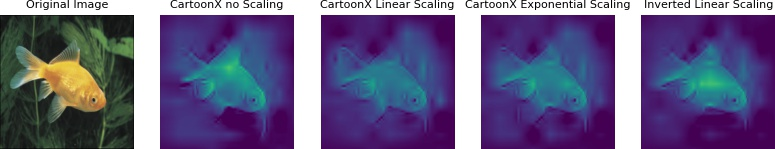
\includegraphics[width=0.85\textwidth]{images/qualitative_ims/obfuscation_examples/goldfish.JPEG}
    \caption{Obfuscation experimentation qualitative results for the image of a goldfish.}
    \label{fig:exp-goldfish}

\end{figure}

This shows that not only was there a reduction in the average distortion with the use of the modified obfuscation method, but there was also a reduction in the overall standard deviation of these distortions relative to the average distortions across all experiments presented. This means that this slight alteration not only improves the overall distortion values, but also produces distortions that are more consistent across different images.

\subsubsection{Applications of  CartoonX}
We use CartoonX to visualize the explanations for several applications namely Semantic Segmentation and object detection.From this we can claim that perhaps CartoonX is task agnostic. One thing common among all these applications is that they are end to end differentiable in nature which allows CartoonX to select the wavelet mask.
\paragraph{Semantic Segmentation}
Using CartoonX we can visualize the explanations specific to the segmentation of a particular class. This allows us to make sure the segmentation network pays attention to right object of the image to predict the segmentation map. From \autoref{fig:segmentation-results} we can see how cartoonX is able to focus on objects of the same class while blurring the others. That is inorder to predict the segmentation of the cow it blurs the cars and viceversa.

\begin{figure}[ht]

\centering
\subfloat[]{\includegraphics[width=0.27\textwidth]{images/Segmentation/Cow_Example/cow.jpg}}\hfil
\subfloat[]{\includegraphics[width=0.27\textwidth]{images/Segmentation/Cow_Example/cow_cow_seg.jpg}}\hfil 
\subfloat[]{\includegraphics[width=0.27\textwidth]{images/Segmentation/Cow_Example/cow_car_seg.jpg}} 

\subfloat[]{\includegraphics[width=0.27\textwidth]{images/Segmentation/Cow_Example/cowgray.jpg}}\hfil   
\subfloat[]{\includegraphics[width=0.27\textwidth]{images/Segmentation/Cow_Example/cow_focus.png}}\hfil
\subfloat[]{\includegraphics[width=0.27\textwidth]{images/Segmentation/Cow_Example/car_focus.png}}
\caption{CartoonX on Image segmentation.}\label{fig:segmentation-results}
\end{figure}






% Fixed :) nice
\paragraph{Object Detection}
Again we qualitatively evaluate CartoonX on the task of Object detection via YOLO \cite{redmon2016you}. From \autoref{fig:Object-results} we can see that CartoonX does well in focusing on the objects of relevance while blurring the background. In the figure CartoonX explanation focuses exactly on the Eagle while blurring the field it is present in. This is as expected because the background is not essential for YOLO to detect the object of interest. 

\begin{figure}[H]

\centering
\subfloat[]{\includegraphics[width=0.27\textwidth]{images/YOLO/eagel2.jpg}}\hfil   
\subfloat[]{\includegraphics[width=0.27\textwidth]{images/YOLO/eagle_ObjectD.png}}\hfil
\subfloat[]{\includegraphics[width=0.27\textwidth]{images/YOLO/eagle_ObjectDCartoon.png}}
\caption{CartoonX on Object Detection.}\label{fig:Object-results}
\end{figure}






\subsubsection{Effect of Network Architecture on the explainations}
As another extension to the original paper, we test CartoonX for different model architectures. We plot the rate-distortion curve by keeping the most relevant coefficients and randomizing the others. The original paper does this for the MobileNetV3 pre-trained on the ImageNet dataset. We extend this for ResNet-18 \cite{he2016deep}, ResNet-50\cite{he2016deep}, and ViT-B/16\cite{dosovitskiy2020image} models. Consecutively, we use the pre-trained models on ImageNet and take the average results for 100 images. \autoref{fig:rate_distortion_archs} shows the results for rate-distortion curves.

% \begin{figure}[H]
%     \centering
%     \includegraphics[width=0.5\textwidth]{images/rate_distortion_archs.png}
%     \caption{Rate-distortion curve for different convolutional and vision transformer architectures.}
%     \label{fig:rate_distortion_archs}
% \end{figure}

\begin{figure}[H]
    \centering
    \subfloat[]{\includegraphics[width=0.3\textwidth]{images/rate_distortion_archs.png}}\hfil
    \subfloat[]{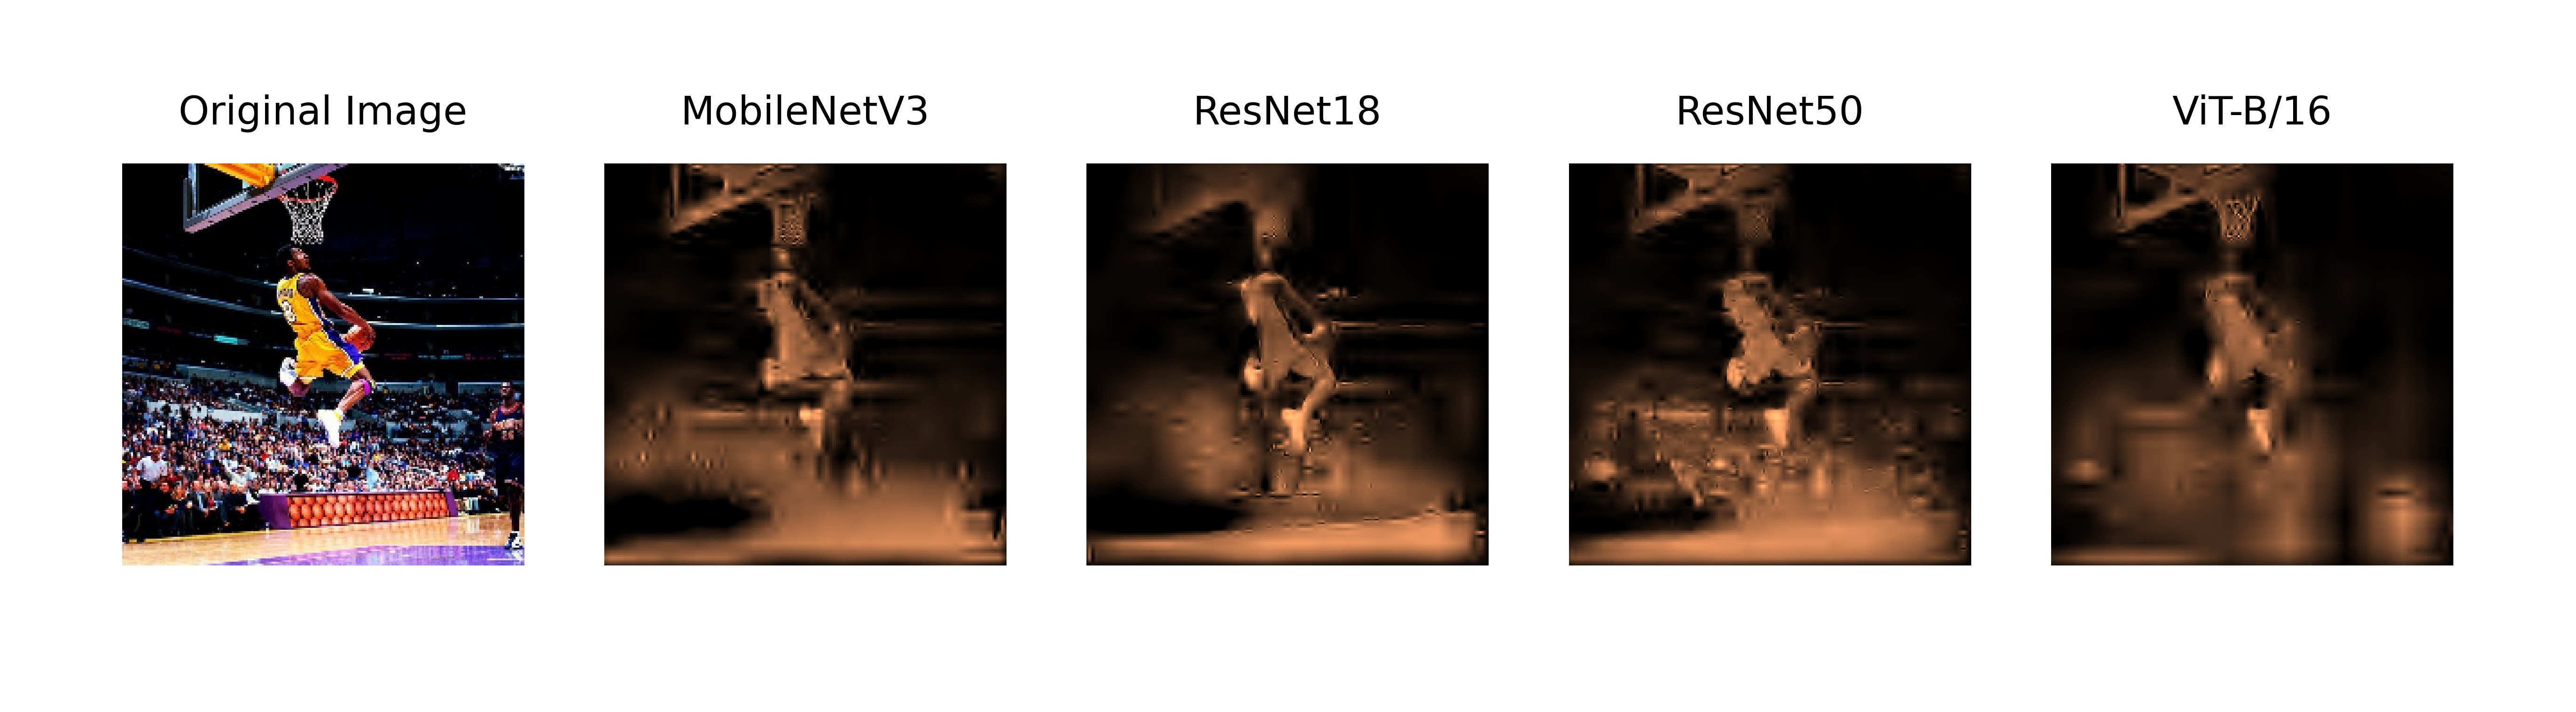
\includegraphics[width=0.6\textwidth]{images/CartoonX_archs.jpeg}}\hfil
    
    \caption{(a) Rate-distortion curve for different convolutional and vision transformer architectures. (b) CartoonX explanations on different model architectures for "basketball" class.}
    \label{fig:rate_distortion_archs}
\end{figure}

We see that different architectures have different rate-distortion values at the beginning, but ResNet and ViT architectures decay faster than MobileNetV3. ViT starts with the most rate-distortion value but also decays fastest. \autoref{fig:rate_distortion_archs} further shows the difference in CartoonX representations for models. For example, for ViT the "basket" is more highlighted, suggesting a possible key point that could show why a model performs better at certain tasks such as classification.



\section{Discussion}\label{sec:discussion}
In order to conduct a proper reproduction of the paper by Kolek et al. we executed several qualitative and quantitative experiments with the goal of also extending on the original work. While the majority of experiments conducted validated the overall reproducibility of the paper, some figures produced results that were not quite as similar to those produced by the original authors initially. Mainly, when conducting the quantitative analysis, we found the only after changing the number of iterations used to create the non-randomized and randomized relevant component distortion plots shown in \autoref{fig:quantitative-results} were the results actually comparable to those produced in the original. Additionally, although the $\lambda$ experimentation produced plots with similar trends as those shown in the original, the results produced, especially those for the PixelRDE, were in fact not similar. This may have been due to the hyperparameters not being clearly specified for this plot . \\

Thanks to the code being provided not only in a very structured manner but also with clear instructions, the initial qualitative results were produced quickly and without any additional scripting.

\subsection{What was easy}
Overall, the initial qualitative result process was easy due to the initial layout of both the repository and the procedures that were presented within the paper. The ease of this process can be specifically attributed to the organization of the repository making it easily navigable, as well as the documentation also provided within the repository, detailing a step-by-step process on installing all dependencies and setting up the code for an initial qualitative run. This led to our ability to add multiple extensions onto the original paper, ultimately adding a layer of robustness to the claims made and the work done by the original authors. 
\subsection{What was difficult}
Some important hyperparameters required to reproduce the quatitative results were missing. The code for multiple baseline methods used for comparison against CartoonX was not provided in the codebase so we had to code them on our own.And also all the hyperparameters for the baselines were not clear making fair comparison a bit difficult. 

\subsection{Communication with original authors}
In order to clarify some points within the quantitative results, some questions were posed to the authors regarding the $\lambda$ values used within the quantitative results. while this did help to clarify some hyperparameters used such as the $\lambda$ values, other questions arose later in the process that were unfortunately left unanswered due to the short timeline provided. One question we did manage to answer independently was how many steps were used to produce some of the quantitative results, specifically those pertaining to the amount of distortion when using a certain portion of randomized and non-randomized components. We found the plots for 100 steps more closely resembling those in the original paper, even though we were unsure about using 2000 steps or 100 steps. 